\documentclass[DIN, pagenumber=false, fontsize=11pt, parskip=half]{scrartcl}

\usepackage{ngerman}
\usepackage[utf8]{inputenc}
\usepackage[T1]{fontenc}
\usepackage{textcomp}

% for matlab code
% bw = blackwhite - optimized for print, otherwise source is colored
\usepackage[framed,numbered,bw]{mcode}

% for other code
%\usepackage{listings}
\usepackage{amssymb}
\usepackage{graphicx}
\graphicspath{ {./imgs/} }

\setlength{\parindent}{0em}

% set section in CM
\setkomafont{section}{\normalfont\bfseries\Large}

\newcommand{\mytitle}[1]{{\noindent\Large\textbf{#1}}}
\newcommand{\mysection}[1]{\textbf{\section*{#1}}}
\newcommand{\mysubsection}[2]{\romannumeral #1) #2}
%===================================
\begin{document}

\noindent\textbf{Financial Computing} \hfill \textbf{National Taiwan University}\\
R14944037 Yu Xiang Luo\\

\mytitle{Assignment 1 \hfill \today}
%===================================
\mysection{Prerequisite}
\begin{itemize}
	\item $\frac{dS}{S} = \mu dt + \sigma dZ$
	\item $ln S_T = ln S_0 + (r - q - \frac{\sigma^2}{2})T + \sigma \Delta Z^Q(T)$
	\item $N(\cdot)$ denotes the CDF of the standard normal distribution.
\end{itemize}
%===================================
\mysection{Basic Requirement}
\[
	\fbox{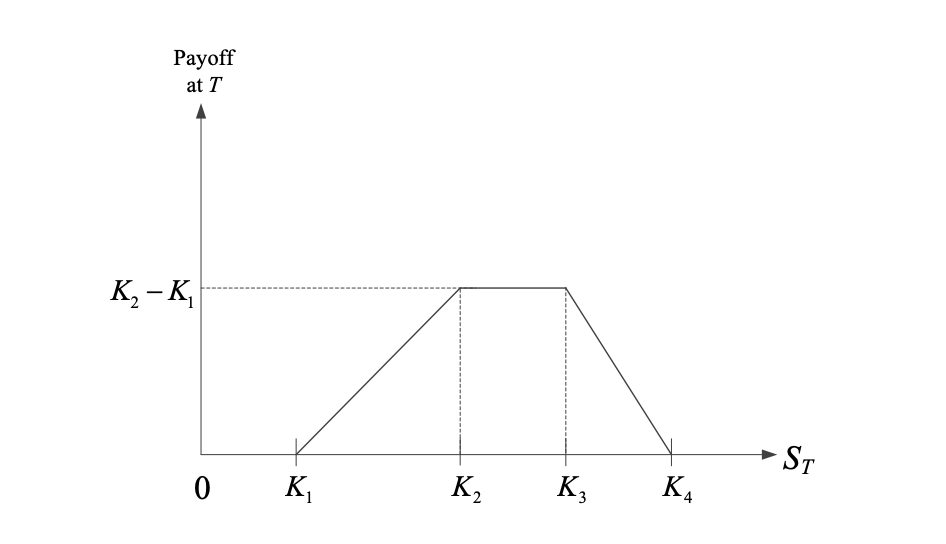
\includegraphics[width=0.5\textwidth]{options}}
\]
\mysubsection{1}{
	\textbf{Derivation of the closed-form formula:} Let $f(S_T)$ be the payoff function. Under the risk-neutral measure $\mathbb{Q}$,
	the asset price $S_T$ follows a lognormal distribution, and the present value of the option is discounted expected payoff:
	$$V_0 = e^{-rT}E^\mathbb{Q}[Payoff(S_T)]$$
	The payoff can be decomposed into three indicator functions $1_{A}$, $1_{B}$, and $1_{C}$:
	$$E^Q[Payoff(S_T)] = E^Q[(S_T - K_1)1_A + (K_2 - K_1)1_B + ((K_2 - K_1) - m(S_T - K_3))1_C]$$
	where $m = \frac{K_2 - K_1}{K_4 - K_3}$ and the events are:
	\begin{itemize}
		\item $A = \{K_1 \leq S_T < K_2\}$
		\item $B = \{K_2 \leq S_T < K_3\}$
		\item $C = \{K_3 \leq S_T < K_4\}$
	\end{itemize}
	For $[K1, K2]$, $E^Q[(S_T - K_1)1_A] = E^Q[S_T \cdot 1_A] - K_1E^Q[1_A]$
	\begin{itemize}
		\item The option is in-the-money if $S_T > K$
			\begin{enumerate}
				\item $S_0e^{(r-q-\frac{1}{2}\sigma^2)T + \sigma\sqrt{T}Z} > K$
				\item $(r-q-\frac{1}{2}\sigma^2)T + \sigma\sqrt{T}Z > \ln\left(\frac{K}{S_0}\right)$
				\item $Z$: $\sigma\sqrt{T}Z > \ln\left(\frac{K}{S_0}\right) - (r-q-\frac{1}{2}\sigma^2)T$
				\item $\sigma\sqrt{T}Z > -\ln\left(\frac{S_0}{K}\right) - (r-q-\frac{1}{2}\sigma^2)T$
				\item $Z > \frac{-\ln(S_0/K) - (r-q-\frac{1}{2}\sigma^2)T}{\sigma\sqrt{T}}$
				\item $Z < \frac{\ln(S_0/K) + (r-q-\frac{1}{2}\sigma^2)T}{\sigma\sqrt{T}}$, By the symmetry of normal distribution
				\item Define $d_2(K) = \frac{\ln(S_0/K) + (r-q-\frac{1}{2}\sigma^2)T}{\sigma\sqrt{T}}$
			\end{enumerate}
	\end{itemize}
	$d_2(K)$ is the probability of $S_T$ reaching $K$. Therefore:
	$$E^Q[1_A] = N(d2(K1)) - N(d2(K2))$$
	To calculate $E^Q[S_T \cdot 1_A]$, we define a Radon-Nikodym derivative $\Lambda = e^{-\frac{\sigma^2}{2}T + \sigma \Delta Z^Q(T)}$ to 
	change from measure $Q$ to measure $R$. Setting $H(t) = -\sigma$ in the Girsanov theorem, the relation between $Q$ and $R$ measure
	would be:
	$$dZ^R = dZ^Q - \sigma dt$$
	The drift term in $R$ measure would change to:
	$$ln S_T = ln S_0 + (r - q + \frac{\sigma^2}{2})T + \sigma \Delta Z^R(T)$$
	$$d_1(K) = \frac{\ln(S_0/K) + (r-q+\frac{1}{2}\sigma^2)T}{\sigma\sqrt{T}}$$
	Applying $E^Q[\Lambda \cdot 1_A] = E^R[1_A]$:
	$$E^Q[S_T \cdot 1_A] = S_0 e^{(r-q)T} N(d_1(K_1)) - S_0 e^{(r-q)T} N(d_1(K_2))$$
	For $[K2, K3]$, the payoff is a constant $K_2 - K_1$. We only need the risk-neutral probability:
	$$E^Q[(K_2 - K_1) 1_B] = (K_2 - K_1) [N(d_2(K_2)) - N(d_2(K_3))]$$
	For $[K3, K4]$, the slope is $m = \frac{K_2-K_1}{K4-K3}$ and the payoff function is $m(K_4-S_T)$
	$$E^Q[m(K_4 - S_T)1_C] = m K_4 E^Q[1_C] - m E^Q[S_T 1_C]$$
	$$E^Q[m(K_4 - S_T)1_C] = m K_4 E^Q[1_C] - m E^Q[S_T 1_C]$$
	Similar to previous $Q \rightarrow R$:
	$$E^Q[m(K_4 - S_T)1_C] = m K_4 [N(d_2(K_3)) - N(d_2(K_4))] - m S_0 e^{(r-q)T} [N(d_1(K_3)) - N(d_1(K_4))]$$
	Finally, add everything and discount by $e^{-rT}$:
	$$V_0 = S_0 e^{-qT} [N(d_1(K_1)) - N(d_1(K_2))] - K_1 e^{-rT} [N(d_2(K_1)) - N(d_2(K_2))]$$
	$$+ (K_2 - K_1) e^{-rT} [N(d_2(K_2)) - N(d_2(K_3))]$$
	$$+ m K_4 e^{-rT} [N(d_2(K_3)) - N(d_2(K_4))] - m S_0 e^{-qT} [N(d_1(K_3)) - N(d_1(K_4))]$$
	Where $N(\cdot)$, $d_1(K)$, $d_2(K)$, and $m$ are:
	$$N(x) = ND(0, 1).cdf(x)$$
	$$d_1(K) = \frac{\ln(S_0/K) + (r-q+\frac{1}{2}\sigma^2)T}{\sigma\sqrt{T}}$$
	$$d_2(K) = \frac{\ln(S_0/K) + (r-q-\frac{1}{2}\sigma^2)T}{\sigma\sqrt{T}}$$
	$$m = \frac{K_2 - K_1}{K_4 - K_3}$$
}
\mysubsection{2}{
	The pseudo code of the program is as follow, the detail python script can be found in supplementary.
}
\begin{lstlisting}
def N(x: float) -> float:
    return NormalDist(0.0, 1.0).cdf(x)

def calc_d1(S0, K, T, r, q, sigma)
    return (
		math.log(S0 / K) 
		+ (r - q + 0.5 * sigma**2) * T) / (sigma * math.sqrt(T)
	)

def calc_d2(d1_val, T, sigma):
    return d1_val - sigma * math.sqrt(T)

# d_K = calc_d(S0, K, T, r, q, sigma)

part1_asset = S0 * math.exp(-q * T) * (N(d1_K1) - N(d1_K2))
part1_cash  = K1 * math.exp(-r * T) * (N(d2_K1) - N(d2_K2))
segment_1   = part1_asset - part1_cash

segment_2 = (K2 - K1) * math.exp(-r * T) * (N(d2_K2) - N(d2_K3))

part3_cash  = m * K4 * math.exp(-r * T) * (N(d2_K3) - N(d2_K4))
part3_asset = m * S0 * math.exp(-q * T) * (N(d1_K3) - N(d1_K4))
segment_3   = part3_cash - part3_asset

V0 = segment_1 + segment_2 + segment_3
\end{lstlisting}
\mysection{Bonus 1}
By reducing the derivation above, we can actually get:
\begin{itemize}
	\item Strike $K_1$ terms: $S_0 e^{-qT} N(d_1(K_1)) - K_1 e^{-rT} N(d_2(K_1)) = \mathbf{C(K_1)}$
	\item Strike $K_2$ terms: $-S_0 e^{-qT} N(d_1(K_2)) + K_1 e^{-rT} N(d_2(K_2)) + (K_2 - K_1) e^{-rT} N(d_2(K_2))$
		\newline
		$\Rightarrow -S_0 e^{-qT} N(d_1(K_2)) + K_2 e^{-rT} N(d_2(K_2)) = \mathbf{-C(K_2)}$
	\item Strike $K_3$ terms: $-(K_2 - K_1) e^{-rT} N(d_2(K_3)) + (K_2 - K_1 + mK_3) e^{-rT} N(d_2(K_3)) - m S_0 e^{-qT} N(d_1(K_3))$
		\newline
		$\Rightarrow mK_3 e^{-rT} N(d_2(K_3)) - m S_0 e^{-qT} N(d_1(K_3)) = \mathbf{-m \cdot C(K_3)}$
	\item Strike $K_4$ terms: $-(K_2 - K_1 + mK_4 - mK_4 + mK_3) e^{-rT} N(d_2(K_4)) + m S_0 e^{-qT} N(d_1(K_4))$
		\newline
		$\Rightarrow m S_0 e^{-qT} N(d_1(K_4)) - m K_4 e^{-rT} N(d_2(K_4)) = \mathbf{m \cdot C(K_4)}$
\end{itemize}
\begin{lstlisting}
# Full script can be found in supplementary
m = (K2 - K1) / (K4 - K3)

c1 = bs_call_price(S0, K1, r, q, sigma, T)
c2 = bs_call_price(S0, K2, r, q, sigma, T)
c3 = bs_call_price(S0, K3, r, q, sigma, T)
c4 = bs_call_price(S0, K4, r, q, sigma, T)

total = c1 - c2 - m * c3 + m * c4

\end{lstlisting}
\mysection{Bonus 2}
The corresponded script can be found in supplementary.
\begin{lstlisting}
Prices = []
Iterate 20 times:
	Price = SimulatePrice(average 10,000 times)
	Prices.append(Price)

Mean, Std = mean(Prices), std(Prices)
Lowerbound, Upperbound = Mean - 2 * Std, Mean + 2 * Std
return Mean, Lowerbound, Upperbound
\end{lstlisting}
\end{document}
